\documentclass[a4paper]{article}
\usepackage[margin=1.5in]{geometry}
\usepackage{listings}
\usepackage[pdftex]{graphicx}



\begin{document}

\textbf{COMP24111 - ex3 - Spam filtering}

\textbf{James W Peach - 8974863}

\section{Parameters}


The parameters I used for the Naive Bayes classifier are as follows:

{\centering\begin{lstlisting}
% Put your NB training function below
[ Classes, Values, Prior, Likelihood ] = NBTrain(AttributeSet, LabelSet);
% Put your NB test function below
[predictLabel, accuracy] = NBTest(Classes, Values, Prior, Likelihood,
	 testAttributeSet, validLabel); % NB test
\end{lstlisting}\par}

\begin{itemize}
\item Classes - This is a convenience variable with the list of classes in the original data set e.g. [2,5,4]
\item Values - This is a convenience variable with the list of Values from the original data set e.g. [5,6,7] 
\item Prior - This is a matrix with the prior probability for each of the classes appearing in any given new example [0.7,0.8,0.5]. $\hat{P}(C=c_i)$
\item Likelihood - This is a 3-dimensional matrix with the probability for each class,feature,value.  $\hat{P}(X_{j} = x_jk | C = c_i)$
\end{itemize}
\section{Feature Extraction}

The above method relies on discrete and possibly continuous features from the body text and subject line of each image, there needs to be an extraction that produces these values from each email in order to use the Naive Bayes classifier.
One such technique I have done some research on is the Markov chain. 
\begin{figure}[h]
\begin{center}
  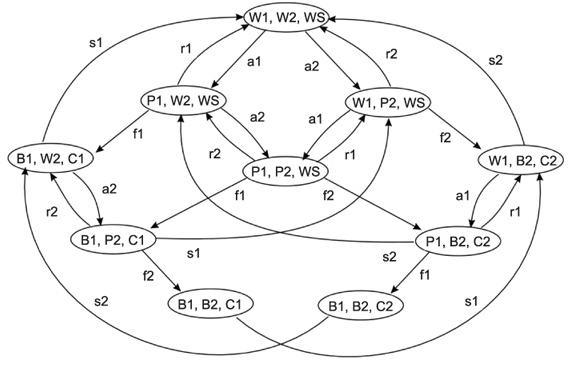
\includegraphics[width=0.48\textwidth]{order-3-markov.jpg}
  \caption{3rd order Markov chain}
\end{center}
\end{figure}
The Markov chain will help identify the context of the words used in the email, other approaches may be a word frequency count or similar this approach will possibly have more false positives than the Markov extraction because it does not take into consideration the words used around.

Finally Principal component analysis will tell us which features and words extracted from the training data are most representative of the classes we want to identify. and which features we should throw away.
\end{document}
